\documentclass[tikz,border=5pt]{standalone}
\usepackage{pgfplots}
\usepackage{amsmath}
\pgfplotsset{compat=1.18}

\begin{document}
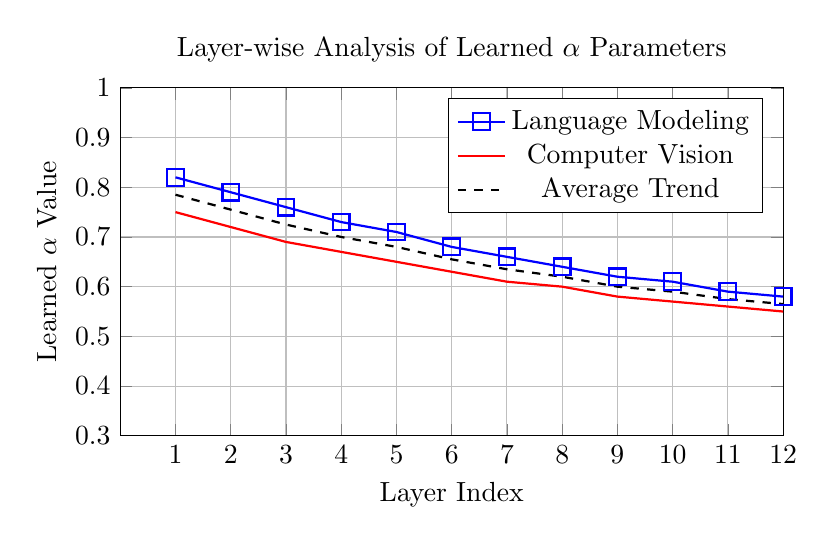
\begin{tikzpicture}
\begin{axis}[
    width=10cm,
    height=6cm,
    xlabel={Layer Index},
    ylabel={Learned $\alpha$ Value},
    title={Layer-wise Analysis of Learned $\alpha$ Parameters},
    grid=major,
    legend pos=north east,
    xmin=0, xmax=12,
    ymin=0.3, ymax=1.0,
    xtick={1,2,3,4,5,6,7,8,9,10,11,12},
    ytick={0.3,0.4,0.5,0.6,0.7,0.8,0.9,1.0},
    mark size=3pt,
]

% Language modeling data (GPT-2)
\addplot[
    color=blue,
    mark=square,
    thick,
] coordinates {
    (1,0.82) (2,0.79) (3,0.76) (4,0.73) (5,0.71) (6,0.68)
    (7,0.66) (8,0.64) (9,0.62) (10,0.61) (11,0.59) (12,0.58)
};

% Computer vision data (ResNet-18)
\addplot[
    color=red,
    mark=circle,
    thick,
] coordinates {
    (1,0.75) (2,0.72) (3,0.69) (4,0.67) (5,0.65) (6,0.63)
    (7,0.61) (8,0.60) (9,0.58) (10,0.57) (11,0.56) (12,0.55)
};

% Average trend line
\addplot[
    color=black,
    mark=none,
    thick,
    dashed,
] coordinates {
    (1,0.785) (2,0.755) (3,0.725) (4,0.700) (5,0.680) (6,0.655)
    (7,0.635) (8,0.620) (9,0.600) (10,0.590) (11,0.575) (12,0.565)
};

\legend{Language Modeling, Computer Vision, Average Trend}

\end{axis}
\end{tikzpicture}
\end{document} 